% \renewcommand{\thechapter}{\Alph{chapter}}
\chapter{Appendix}
\label{ap:appendix}

\section{Configurations for \texorpdfstring{\ctapipe{}}{ctapipe}}
\label{ap:config_files}

The listing below shows the configuration file used for preprocessing the datasets, \ie{} before the
application of the different cleaning settings.
\begin{spacing}{0.5}
    \begin{mdframed}[backgroundcolor=codebg, hidealllines=true, leftmargin=0cm,rightmargin=0cm, skipabove=0pt, innerleftmargin=0,innerrightmargin=0,]
    \lstinputlisting[basicstyle=\lstsansserif, language=yaml]{./configs/preprocessing.yml}
    \end{mdframed}
\end{spacing}

The listings below show the contents of the default configuration files used with \ctapipe{}
for each cleaning algorithm respectively.
\begin{description}
    \item \textbf{\tailcuts{}}:\medskip
    \begin{spacing}{0.5}
        \begin{mdframed}[backgroundcolor=codebg, hidealllines=true, leftmargin=0cm,rightmargin=0cm, skipabove=0pt, innerleftmargin=0,innerrightmargin=0,]
        \lstinputlisting[basicstyle=\lstsansserif, language=yaml]{./configs/tailcuts_clean_config.yml}
        \end{mdframed}
    \end{spacing}

    \item \textbf{\mars{}}:\medskip
    \begin{spacing}{0.5}
        \begin{mdframed}[backgroundcolor=codebg, hidealllines=true, leftmargin=0cm,rightmargin=0cm, skipabove=0pt, innerleftmargin=0,innerrightmargin=0,]
        \lstinputlisting[basicstyle=\lstsansserif, language=yaml]{./configs/mars_cleaning_1st_pass_config.yml}
        \end{mdframed}
    \end{spacing}

    \item \textbf{\fact{}}:\medskip
    \begin{spacing}{0.5}
        \begin{mdframed}[backgroundcolor=codebg, hidealllines=true, leftmargin=0cm,rightmargin=0cm, skipabove=0pt, innerleftmargin=0,innerrightmargin=0,]
        \lstinputlisting[basicstyle=\lstsansserif, language=yaml]{./configs/fact_image_cleaning_config.yml}
        \end{mdframed}
    \end{spacing}

    \item \textbf{\tcc{}}:\medskip
    \begin{spacing}{0.5}
        \begin{mdframed}[backgroundcolor=codebg, hidealllines=true, leftmargin=0cm,rightmargin=0cm, skipabove=0pt, innerleftmargin=0,innerrightmargin=0,]
        \lstinputlisting[basicstyle=\lstsansserif, language=yaml]{./configs/time_constrained_cleaning_config.yml}
        \end{mdframed}
    \end{spacing}
\end{description}

The following listing shows the contents of the \texttt{prod5b\_lapalma\_alpha.yml} configuration file,
which is used to set the allowed telescope IDs for \ctapipe{}\texttt{-process}.
\begin{spacing}{0.5}
    \begin{mdframed}[backgroundcolor=codebg, hidealllines=true, leftmargin=0cm,rightmargin=0cm, skipabove=0pt, innerleftmargin=0,innerrightmargin=0,]
    \lstinputlisting[basicstyle=\lstsansserif, language=yaml]{./configs/prod5b_lapalma_alpha.yml}
    \end{mdframed}
\end{spacing}

Since the comparison of the cleaning algorithms also required differentiating between \glspl{mst}
and \glspl{lst}, the following two listings show the contents of the \texttt{prod5b\_lapalma\_mst.yml} and
\texttt{prod5b\_lapalma\_lst.yml} configuration files, respectively:
\begin{description}
    \item \textbf{\glspl{mst}}:\medskip
    \begin{spacing}{0.5}
        \begin{mdframed}[backgroundcolor=codebg, hidealllines=true, leftmargin=0cm,rightmargin=0cm, skipabove=0pt, innerleftmargin=0,innerrightmargin=0,]
        \lstinputlisting[basicstyle=\lstsansserif, language=yaml]{./configs/prod5b_lapalma_mst.yml}
        \end{mdframed}
    \end{spacing}

    \item \textbf{\glspl{lst}}:\medskip
    \begin{spacing}{0.5}
        \begin{mdframed}[backgroundcolor=codebg, hidealllines=true, leftmargin=0cm,rightmargin=0cm, skipabove=0pt, innerleftmargin=0,innerrightmargin=0,]
        \lstinputlisting[basicstyle=\lstsansserif, language=yaml]{./configs/prod5b_lapalma_lst.yml}
        \end{mdframed}
    \end{spacing}
\end{description}


\section{Hyperparameters}
\label{ap:hyperparameters}

The following table shows the subsets of hyperparameters used in the grid search:

\begin{table}
    \centering
    \caption{Hyperparameters for the cleaning algorithms used in the grid search. The picture quantiles
    determine what percent of all pixels per event will be below the core threshold \(Q_c\).
    The boundary threshold is calculated by multiplying the core threshold by the boundary threshold ratio.
    The time limit \(t\) is the parameter for \fact, while the time limits \(t_c\) and \(t_b\) are
    the time limits for \tcc.}
    \label{tab:hyperparameters_gridsearch}
    \rowcolors{0}{white!92!black}{}
    \adjustbox{varwidth=\linewidth,scale=0.9}{%
    \begin{tabular}{
        S[table-format=1.4] S[table-format=1.2] S[table-format=1.0]
        S[table-format=2.1] S[table-format=2.1] S[table-format=2.1]}
        \hiderowcolors
        {Picture Quantiles} & {Boundary Threshold Ratio} & {Minimum Neighbors} &
        {\(t\;/\;\si{\nano\second}\)} & {\(t_c\;/\;\si{\nano\second}\)} & {\(t_b\;/\;\si{\nano\second}\)} \\
        \showrowcolors
        0.995  & 0.25 & 1 &  1.0 &  9.0 &  4.5 \\
        0.999  & 0.33 & 2 &  2.0 & 12.0 &  9.0 \\
        0.9992 & 0.5  & 3 &  4.0 & 15.0 & 12.0 \\
        0.9995 & 0.66 & 4 &  5.0 & 18.0 & 15.0 \\
        0.9997 & 0.75 & 5 &  6.0 & 20.0 & \\
        0.9999 &      &   & 10.0 &      & \\
               &      &   & 12.0 &      & \\
    \end{tabular}}
\end{table}

\section{Software Used}
\label{ap:software}
This work was written and built with \LaTeX{} and Lua\TeX{} from \TeX Live 2021 on both the Windows Subsystem for Linux (WSL, Ubuntu 20.04) on Windows 10 and Ubuntu 20.04.
Also, I relied heavily on the python programming language, of which the most important libraries used
for this work are listed below.
\begin{itemize}
    \item \numpy{}~\cite{numpy}
    \item \pandas{}~\cite{pandas}
    \item \matplotlib{}~\cite{matplotlib}
    \item \astropy{}~\cite{astropy1, astropy2}
    \item \pyirf{}~\cite{pyirf}
    \item \sklearn{}~\cite{scikit-learn}
\end{itemize}

For the processing of the datasets, I used the development version of \texttt{ctapipe}, more specifically,
the code from the \texttt{master} branch from July 6 (\texttt{f26107fe}). A complete listing of all used python libraries can be found below:
\begin{spacing}{0.5}
    \begin{mdframed}[backgroundcolor=codebg, hidealllines=true, leftmargin=0cm,rightmargin=0cm, skipabove=0pt, innerleftmargin=0,innerrightmargin=0,]
    \lstinputlisting[basicstyle=\footnotesize\lstsansserif, multicols=2, language=yaml]{./configs/env.yml}
    \end{mdframed}
\end{spacing}


\section{Additional Plots and Tables}
\label{ap:additional_plots_tables}

\subsection{Metrics}
\label{ap:metrics}
\autoref{tab:metrics} below shows the metrics used in this work as well as their formulas. Also shown is a confusion matrix for
a binary (positive/negative) classification problem.

\glsreset{tpr}\glsreset{fpr}\glsreset{tnr}\glsreset{tp}\glsreset{fn}\glsreset{fp}\glsreset{tn}
\begin{table}
    \centering
    \caption{The metrics used for this works analysis as well as their calculation. Right: Confusion
    matrix for a binary (positive/negative) classification.}
    \label{tab:metrics}
    \begin{subtable}{0.48\textwidth}
        \centering
        \rowcolors{0}{white!92!black}{}
        \adjustbox{varwidth=\linewidth,scale=0.9}{%
        \begin{tabular}{l c}
            \hiderowcolors
            {Metric} & {Calculation} \\
            \showrowcolors
            \gls{tpr} & ${\frac{\tp}{\tp + \fn}}$ \\
            % \gls{fpr} & ${\frac{\fp}{\fp + \tn}}$ \\
            \gls{tnr} & ${\frac{\tn}{\tn + \fp}}$ \\
            \gls{fnr} & ${\frac{\fn}{\fn + \tp}}$ \\
            % \gls{ppv} & ${\frac{\tp}{\tp + \fp}}$ \\
            \gls{acc} & ${\frac{\tp + \tn}{\tp + \fp + \tn + \fn}}$ \\
            \gls{ba} & ${\frac{\tpr + \tnr}{2}}$ \\
        \end{tabular}}
    \end{subtable}%
    \begin{subtable}{0.48\textwidth}
        \centering
        \adjustbox{varwidth=\linewidth,scale=0.85}{%
        \begin{tabular}{r l c c}
            & & \multicolumn{2}{c}{Prediction} \\
            & & positive & negative \\
            \parbox[t]{2mm}{\multirow{2}{*}{\rotatebox[origin=c]{90}{Label}}} &  pos. & \colorbox{white!92!black}{\gls{tp}} & \gls{fn} \\
            & neg. & \gls{fp} & \colorbox{white!92!black}{\gls{tn}} \\
        \end{tabular}}
    \end{subtable}%
\end{table}

\subsection{A comparison of the last steps of the cleaning algorithms}
\label{ap:comparing_last_steps}

\autoref{fig:cleaners_together} below shows the last steps of the cleaning algorithms \tailcuts{}, \mars{}, \fact{} and \tcc{}
for the default parameters set in \ctapipe{}.

\begin{figure}
    \centering
    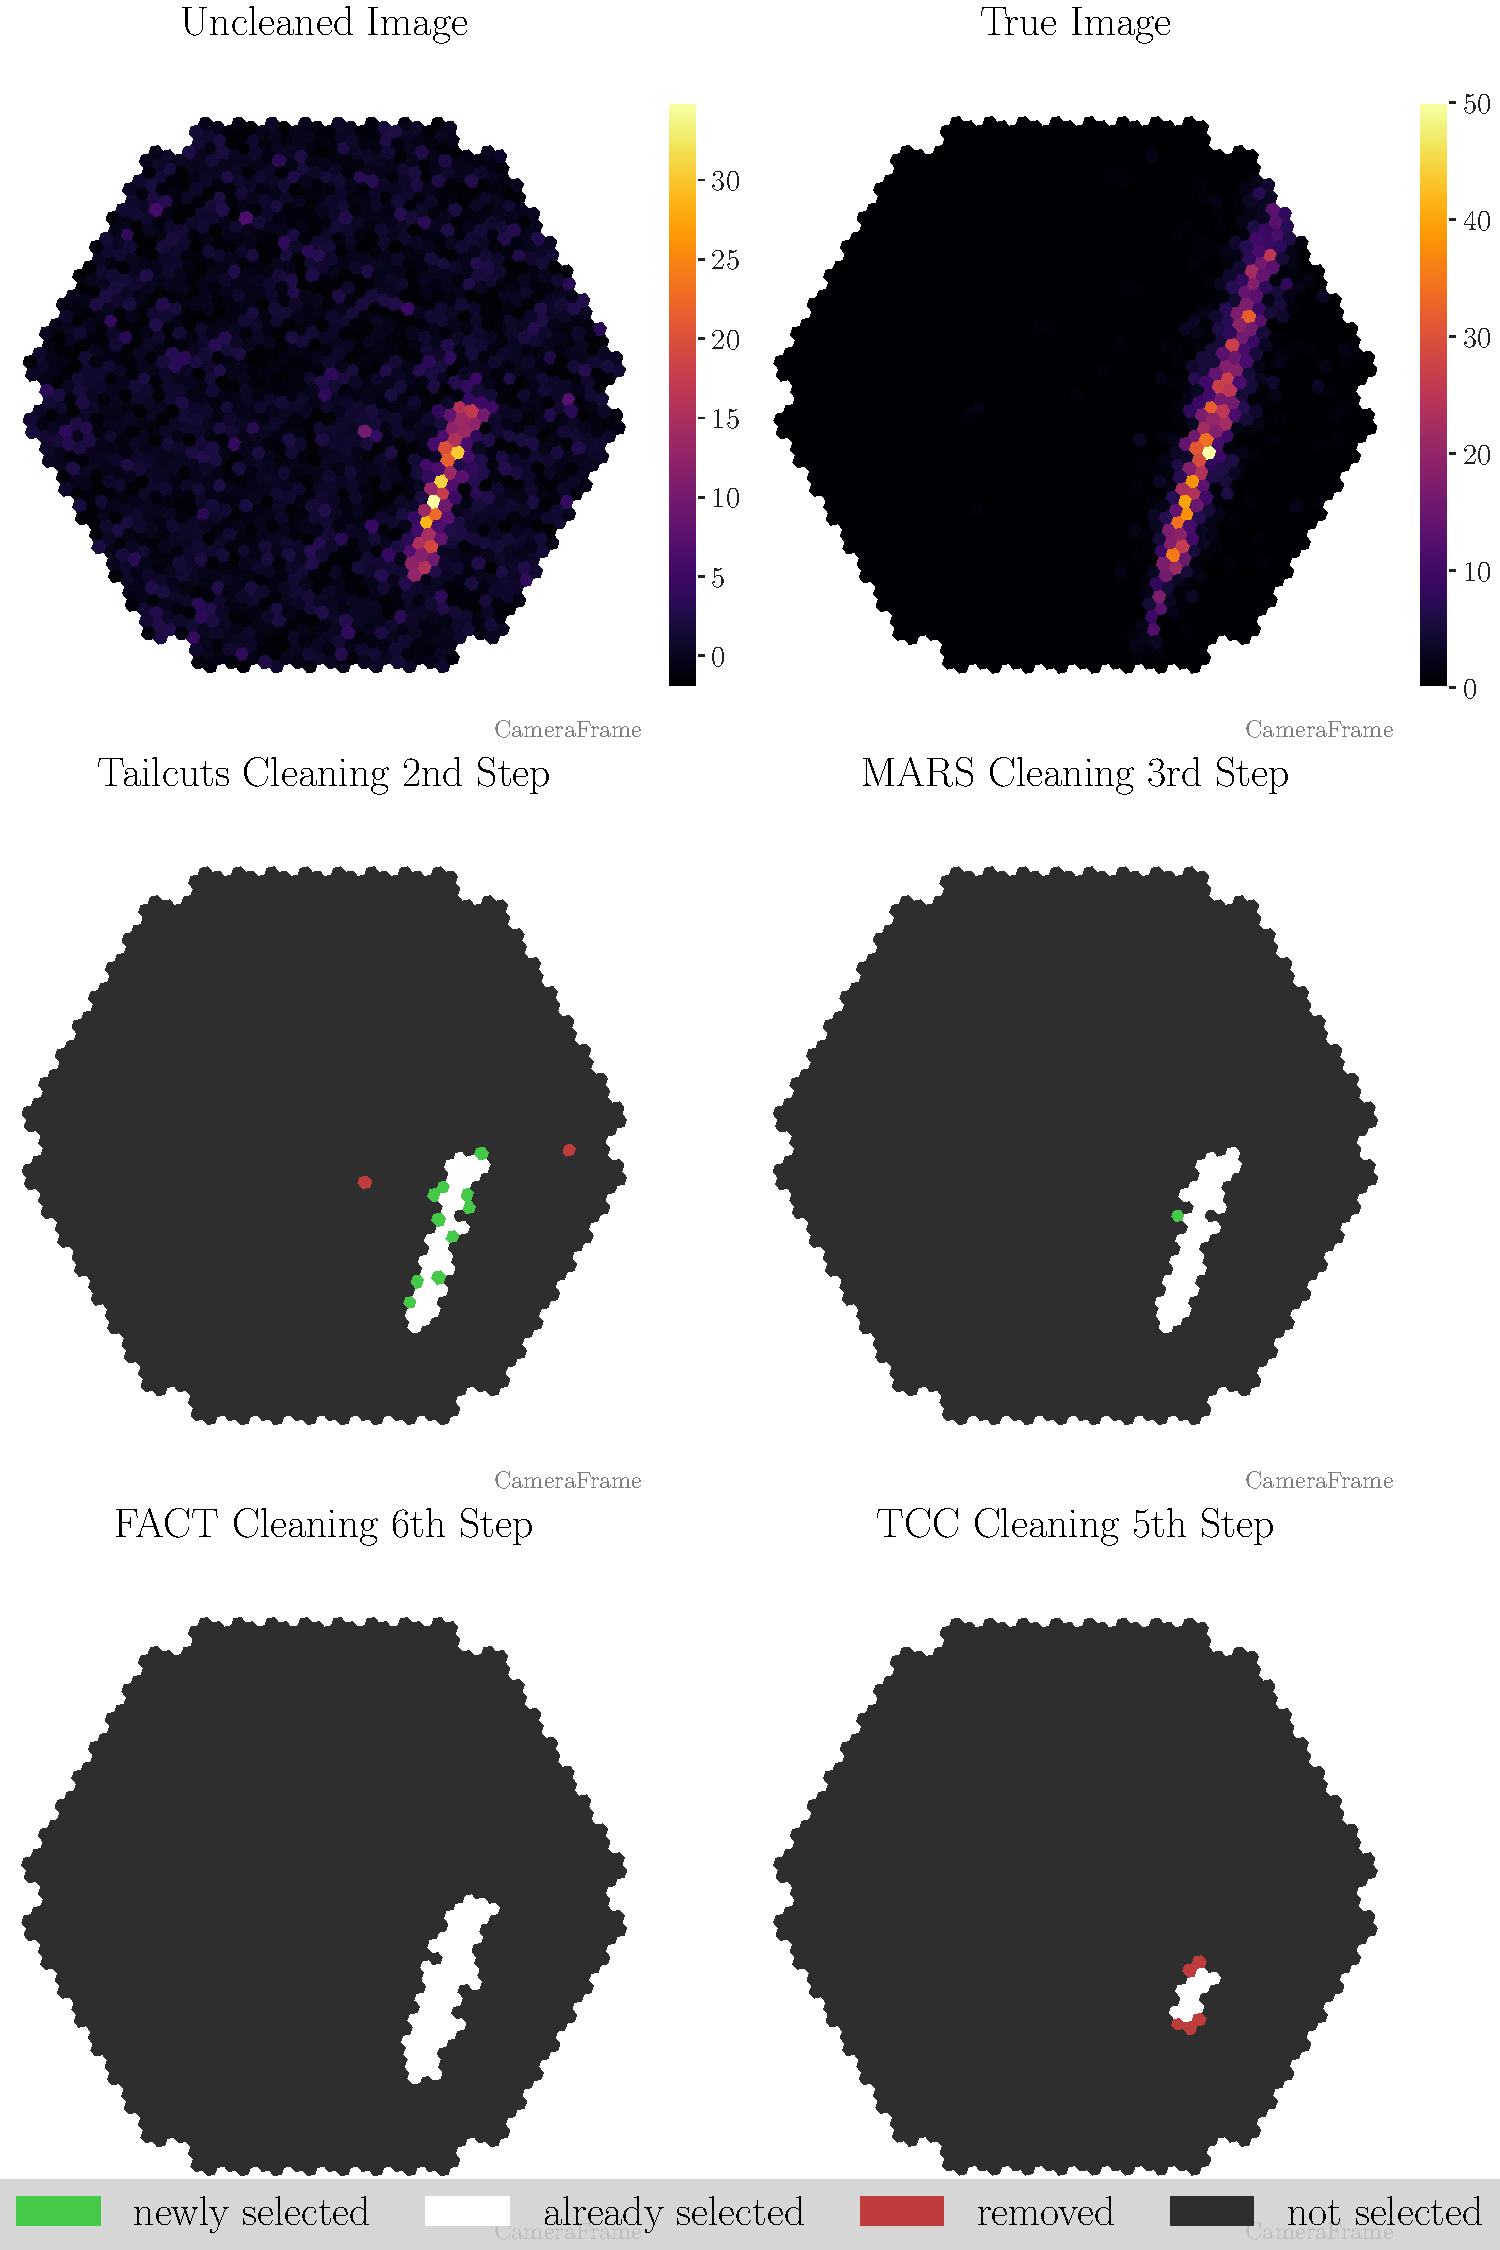
\includegraphics[width=0.65\textwidth]{plots/cleaner_steps/last_steps.pdf}
    \caption{The last steps of the cleaning algorithms \tailcuts{}, \mars{}, \fact{} and \tcc{} for the default
    parameters set in \ctapipe{}. Also shown are the uncleaned image and the true image for better comparison.}
    \label{fig:cleaners_together}
\end{figure}


\subsection{Resulting Settings for Every Cleaning Algorithm}
\label{ap:cleaning_settings_all}

\autoref{tab:zenbu_no_parametoru} below shows all settings determined for every cleaning algorithm. Additionally, the
angular resolution and the efficiency are shown to help with selecting the best settings for a user's needs.
\begin{table}
    \centering
    \caption{All resulting settings for all four cleaning algorithm.
    Listed are the core threshold \(Q_c\), the boundary threshold \(Q_b\),
    the minimum number of neighbors and, where applicable, the time limit \(t\) as well as the core and boundary time limits
    \(t_c\) and \(t_b\). Besides this, the angular resolution and the efficiency are also shown.}
    \label{tab:zenbu_no_parametoru}
    \rowcolors{0}{white!92!black}{}
    \adjustbox{varwidth=\linewidth,scale=0.85}{%
    \begin{tabular}{c S[table-format=2.0] S[table-format=1.3]
        S[table-format=1.3] S[table-format=1.0] S[table-format=2.1] S[table-format=2.1]
        S[table-format=2.1] S[table-format=1.3] S[table-format=1.3]}
        \hiderowcolors
        {Cleaning Algorithm} & {ID} & {\(Q_c \;/\; \si{\pe}\)} & {\(Q_b \;/\; \si{\pe}\)} & {Min. Neigh.} &
        {\(t \;/\; \si{\nano\second}\)} & {\(t_c \;/\; \si{\nano\second}\)} & {\(t_b \;/\; \si{\nano\second}\)} &
        {\(\eff\)} & {Mean Ang. Res\(\;/\; \si{\degree}\)}\\
        \addlinespace[0.5em]
        \showrowcolors
        \tailcuts &  118 & 9.500 & 4.750 & 5 &      &      &      & 0.121 & 0.358 \\
                 &   51 & 9.500 & 6.333 & 4 &      &      &      & 0.177 & 0.308 \\
                 &  140 & 9.500 & 6.333 & 3 &      &      &      & 0.242 & 0.334 \\
                 &  141 & 9.500 & 6.333 & 2 &      &      &      & 0.296 & 0.346 \\
                 &   81 & 9.500 & 4.750 & 2 &      &      &      & 0.307 & 0.357 \\
                 &   47 & 6.200 & 4.650 & 2 &      &      &      & 0.365 & 0.395 \\
                 &  101 & 6.700 & 1.675 & 1 &      &      &      & 0.401 & 0.432 \\
        \addlinespace[0.5em]
        \mars    &   54 & 9.500 & 7.125 & 5 &      &      &      & 0.122 & 0.291 \\
                 &   59 & 9.500 & 6.333 & 4 &      &      &      & 0.179 & 0.282 \\
                 &   76 & 9.500 & 6.333 & 3 &      &      &      & 0.244 & 0.332 \\
                 &   60 & 9.500 & 7.125 & 2 &      &      &      & 0.297 & 0.356 \\
                 &  135 & 9.500 & 6.333 & 2 &      &      &      & 0.306 & 0.343 \\
                 &   15 & 6.700 & 4.467 & 1 &      &      &      & 0.380 & 0.395 \\
                 &   13 & 5.500 & 1.833 & 2 &      &      &      & 0.410 & 0.424 \\
        \addlinespace[0.5em]
        \fact    &  553 & 9.500 & 6.333 & 5 &  2.0 &      &      & 0.007 & 0.244\\
                 &  271 & 9.500 & 4.750 & 4 &  4.0 &      &      & 0.051 & 0.428\\
                 &  767 & 9.500 & 6.333 & 3 &  5.0 &      &      & 0.141 & 0.415\\
                 &  722 & 9.500 & 3.167 & 3 &  5.0 &      &      & 0.178 & 0.367\\
                 &  865 & 9.500 & 7.125 & 2 &  2.0 &      &      & 0.250 & 0.403\\
                 &  691 & 9.500 & 7.125 & 2 &  4.0 &      &      & 0.254 & 0.366\\
                 &  608 & 9.500 & 4.750 & 1 &  6.0 &      &      & 0.340 & 0.365\\
                 &  503 & 6.700 & 3.350 & 1 & 12.0 &      &      & 0.388 & 0.404\\
                 &  974 & 4.200 & 1.400 & 2 &  6.0 &      &      & 0.405 & 0.420\\
        \addlinespace[0.5em]
        \tcc     &   11 & 9.500 & 6.333 & 5 &      & 15.0 & 15.0 & 0.070 & 0.413\\
                 &  367 & 9.500 & 7.125 & 4 &      & 20.0 & 12.0 & 0.121 & 0.396\\
                 &  399 & 9.500 & 6.333 & 3 &      & 18.0 & 12.0 & 0.176 & 0.340\\
                 &  582 & 9.500 & 7.125 & 2 &      & 20.0 & 12.0 & 0.248 & 0.388\\
                 &  171 & 5.700 & 4.275 & 3 &      & 18.0 &  4.5 & 0.263 & 0.386\\
                 & 1495 & 4.200 & 2.800 & 3 &      & 15.0 & 15.0 & 0.311 & 0.383\\
                 &  807 & 6.700 & 4.467 & 1 &      & 15.0 & 12.0 & 0.375 & 0.390\\
                 & 1954 & 6.700 & 1.675 & 1 &      & 15.0 &  9.0 & 0.401 & 0.427\\
    \end{tabular}}
\end{table}